\subsection{CFG Building}
A control flow graph (CFG) is composed of basic blocks. Each basic block contains a sequence of statements that can be executed sequentially. Listing \ref{listing:cfg} illustrates the design of CFG and the building context. High level implementations are shown in following figures.

\begin{lstlisting}[language = python, caption={CFG Design and its building context}, label={listing:cfg}]
  class Block(Visitee):
      def __init__(self, id, name,
                  stmts,  # list of statements in the block
                  cond,   # branching condition

                  next,   # next block on no condition

                  true,   # branched block on true condition
                  false,  # branched block on false condition

                  jump,   # jumped block on FuncCall or CallStmt
                  link,   # linked block after FuncCall or CallStmt
                  end,    # the block ending a FuncCall or CallStmt
                ):
          # Initialization
  
  class CFG(Visitee):
      def __init__(self, blocks, avail_id):
          # Initialization
          
          self.obj.blocks = [Block(id=0)]
  
          # context
          self.ctx.active_block = self.obj.blocks[-1] # any statements rather than IfStmt, WhileStmt and CallStmt will be added to this block when visited
  
          self.ctx.loop_block = None # , active_block points to this block if ContinueStmt is visited
  
          self.ctx.endloop_block = None # pointed to by a visited BreakStmt.

  class CFGBuilderContext:
      def __init__(self, 
                  active_block, # current active block
                  loop_block,   # the first block when entering a loop
                  endloop_block # the block after visit statements in loop
                  ):
          # Initialization
\end{lstlisting}

\begin{figure}
  \centering
  \begin{minipage}{0.45\textwidth}
    \begin{lstlisting}[language=python]
    # Last Block
    if (expr)
      tstmt
    else
      fstmt
    # Next Block
    \end{lstlisting}
  \end{minipage}%
  \hfill
  \begin{minipage}{0.45\textwidth}
    \centering
    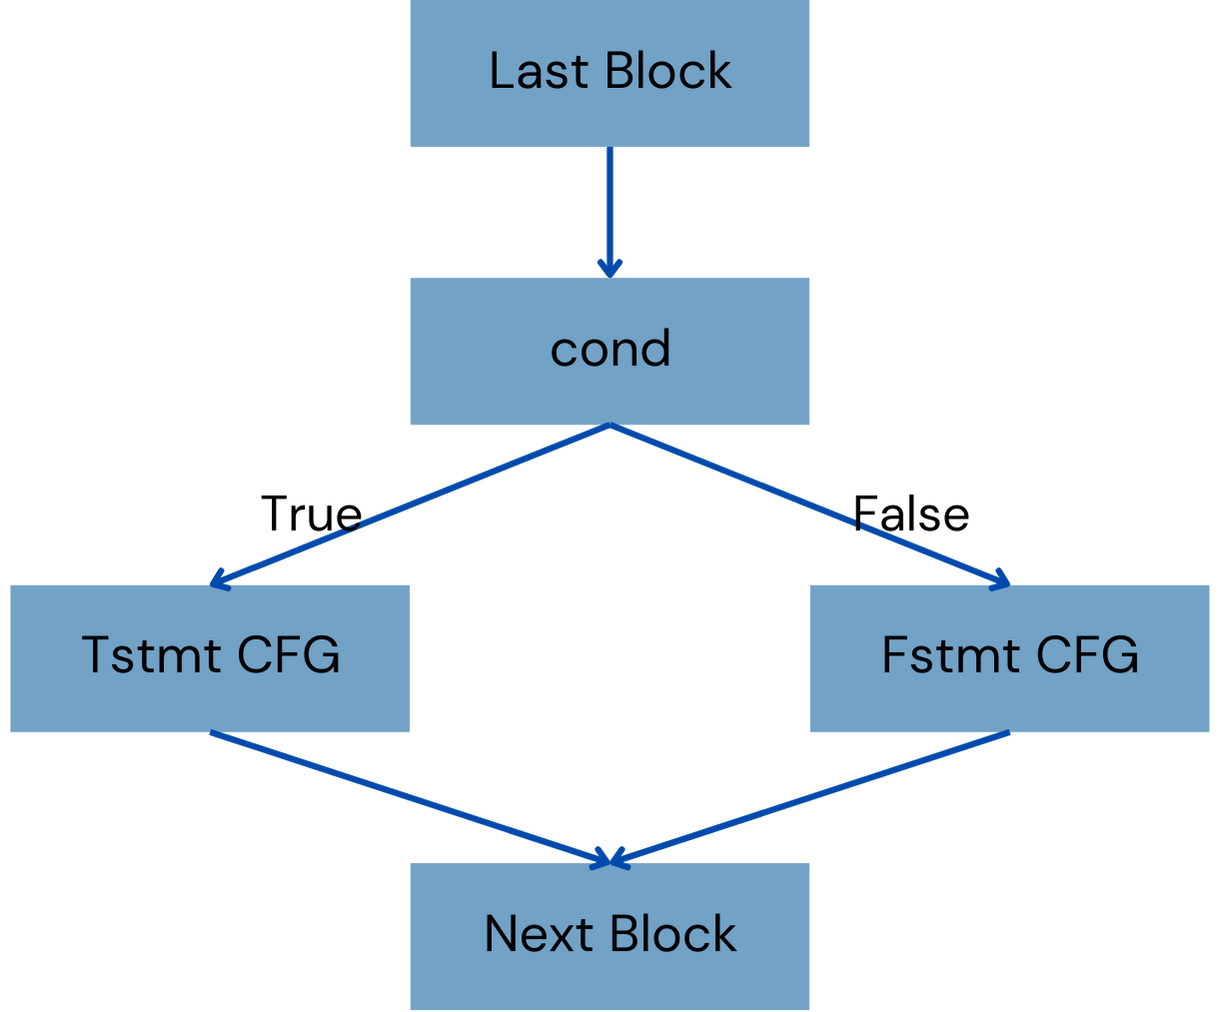
\includegraphics[width=0.9\textwidth]{img/ifstmt-cfg.png}
  \end{minipage}
  \caption{CFG of IfStmt}
\end{figure}

\begin{figure}
  \centering
  \begin{minipage}{0.45\textwidth}
    \begin{lstlisting}[language=python]
    # Last Block
    while (cond) {
      stmt
    }
    # Next Block
    \end{lstlisting}
  \end{minipage}%
  \hfill
  \begin{minipage}{0.225\textwidth}
    \centering
    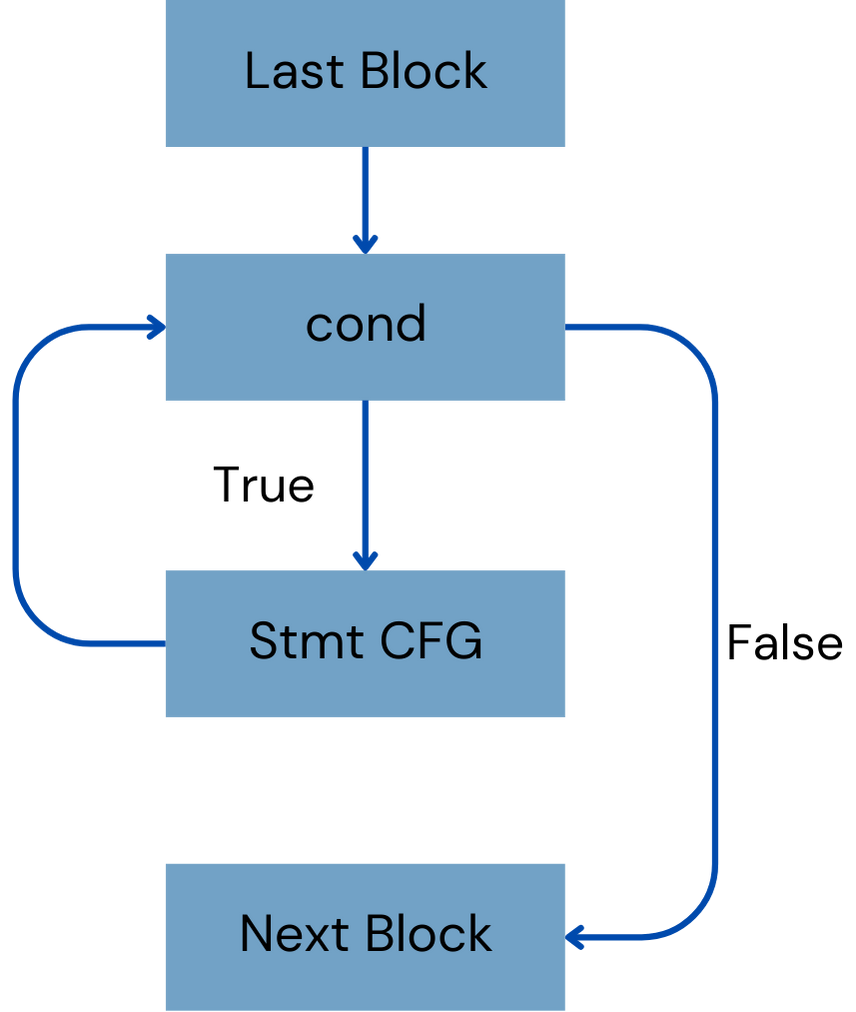
\includegraphics[width=0.9\textwidth]{img/whilestmt-cfg.png}
  \end{minipage}
  \caption{CFG of WhileStmt}
\end{figure}

\begin{figure}
  \centering
  \begin{minipage}{0.45\textwidth}
    \begin{lstlisting}[language=python]
    # Last Block
    do {
      stmt
    } while (cond)
    # Next Block
    \end{lstlisting}
  \end{minipage}%
  \hfill
  \begin{minipage}{0.225\textwidth}
    \centering
    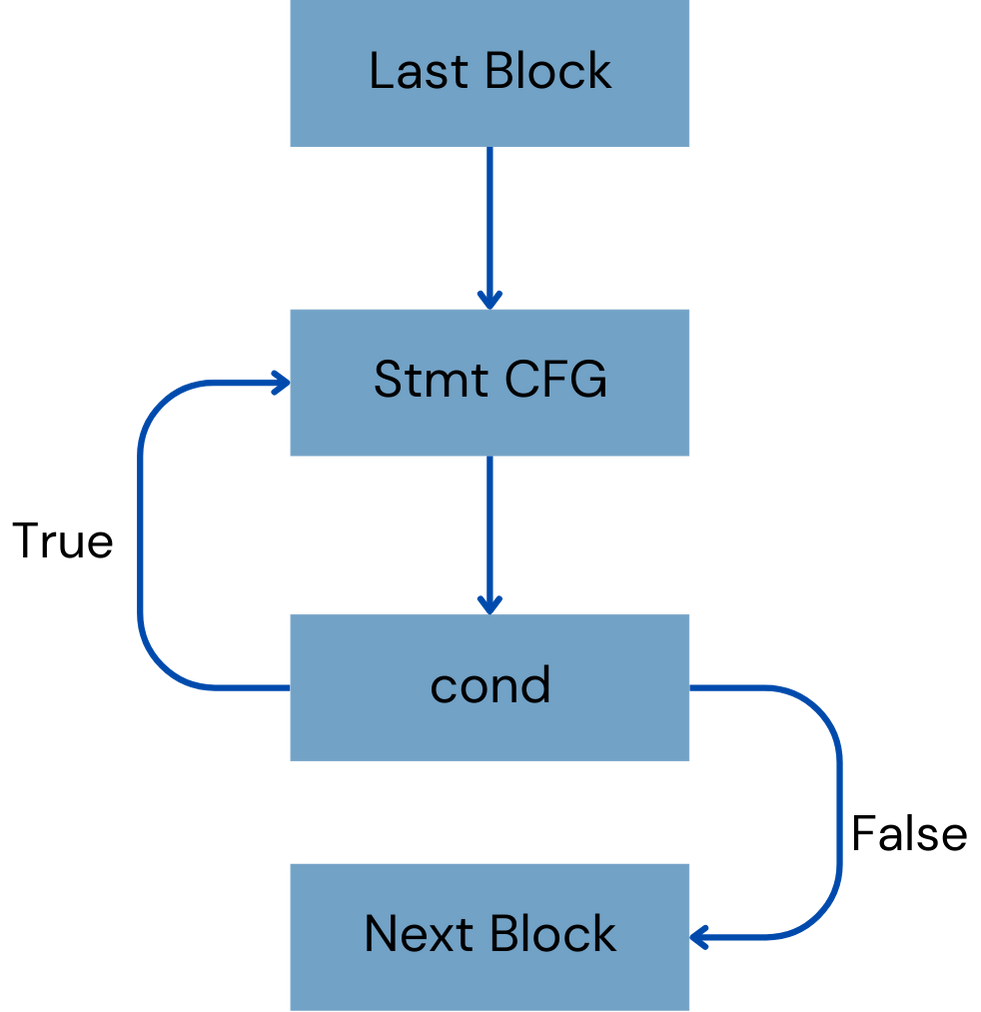
\includegraphics[width=0.9\textwidth]{img/dowhilestmt-cfg.png}
  \end{minipage}
  \caption{CFG of DoWhileStmt}
\end{figure}

% \begin{figure}
%   \centering
%   \begin{minipage}{0.45\textwidth}
%     \begin{lstlisting}[language=python]
%     # Last Block
%     for (assign, cond, update){
%       stmt
%     }
%     # Next Block
%     \end{lstlisting}
%   \end{minipage}%
%   \hfill
%   \begin{minipage}{0.225\textwidth}
%     \centering
%     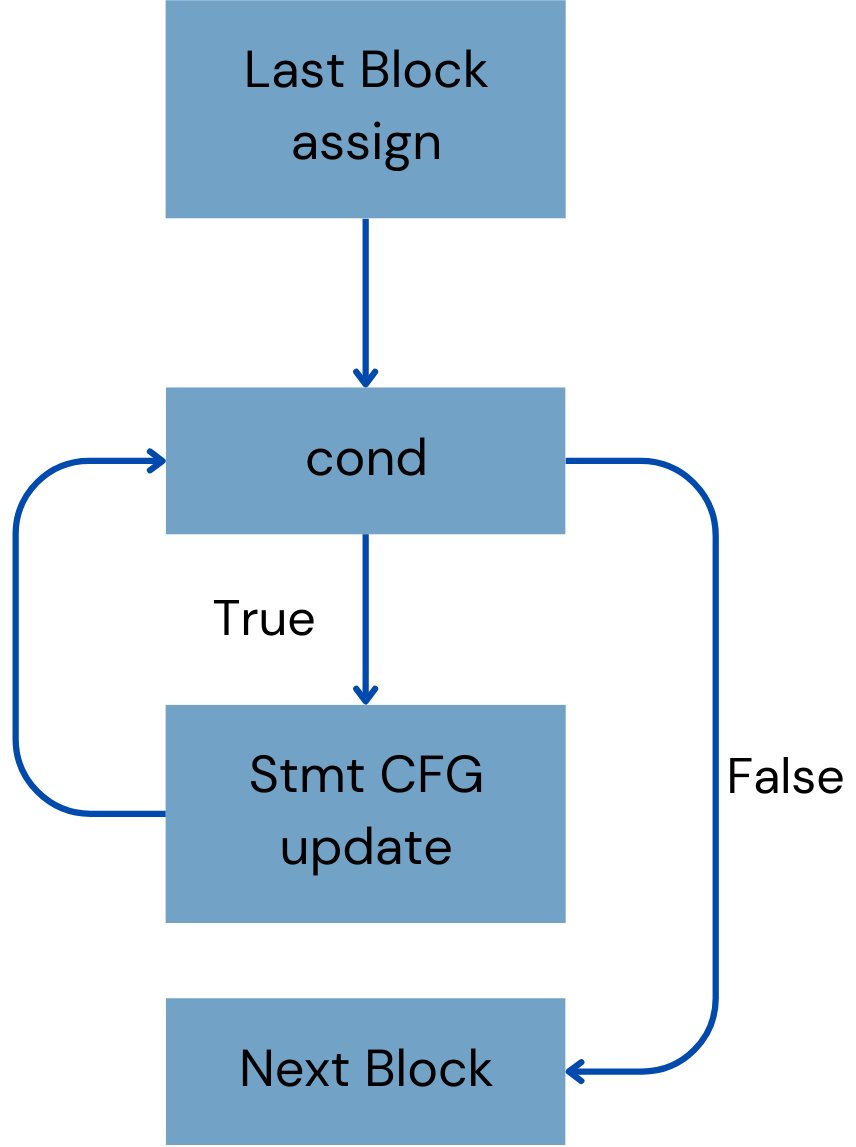
\includegraphics[width=0.9\textwidth]{img/forstmt-cfg.png}
%   \end{minipage}
%   \caption{CFG of ForStmt}
% \end{figure}

\begin{figure}
  \centering
  \begin{minipage}{0.45\textwidth}
    \begin{lstlisting}[language=python]
      func_name : function void ()
        body
      \end{lstlisting}
  \end{minipage}%
  \hfill
  \begin{minipage}{0.45\textwidth}
    \centering
    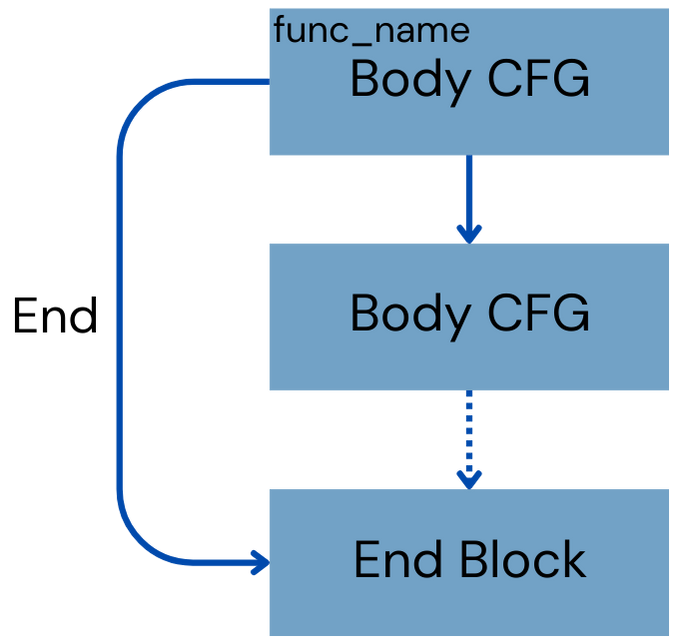
\includegraphics[width=0.5\textwidth]{img/funcdecl-cfg.png}
  \end{minipage}
  \caption{CFG of FuncDecl}
\end{figure}


\begin{figure}[ht]
  \centering
  \centering
  \begin{minipage}{0.45\textwidth}
    \begin{lstlisting}[language=python]
      # Last Block
      func_name(params)
      # Next Block
      \end{lstlisting}
  \end{minipage}%
  \hfill
  \begin{minipage}{0.45\textwidth}
    \centering
    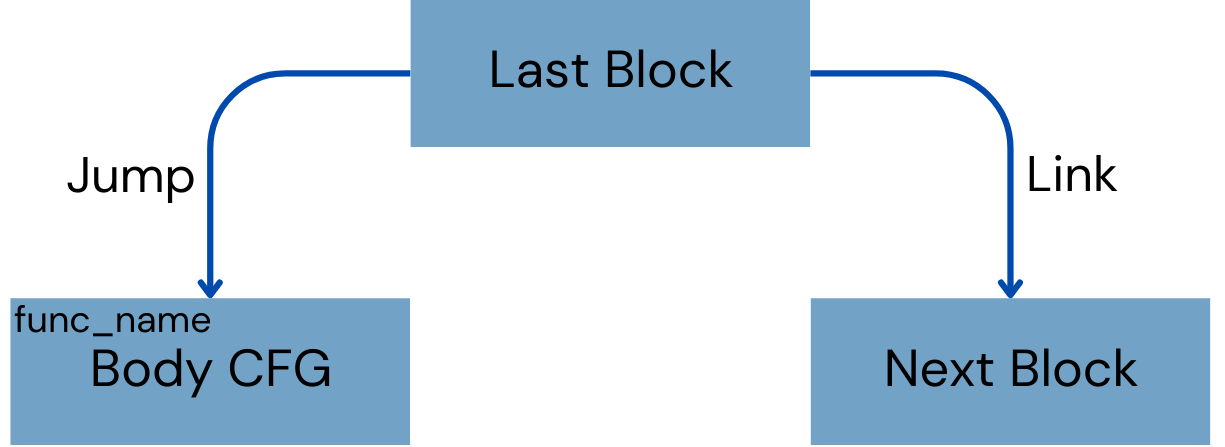
\includegraphics[width=0.9\textwidth]{img/call-cfg.png}
  \end{minipage}
  \caption{CFG of FuncCall and CallStmt}
\end{figure}

We see the structure of a CFG in Figure \ref{figure:cfg-structure}, much simpler than AST in statement types but dataflow expressible.

\begin{figure}[ht]
  \centering
  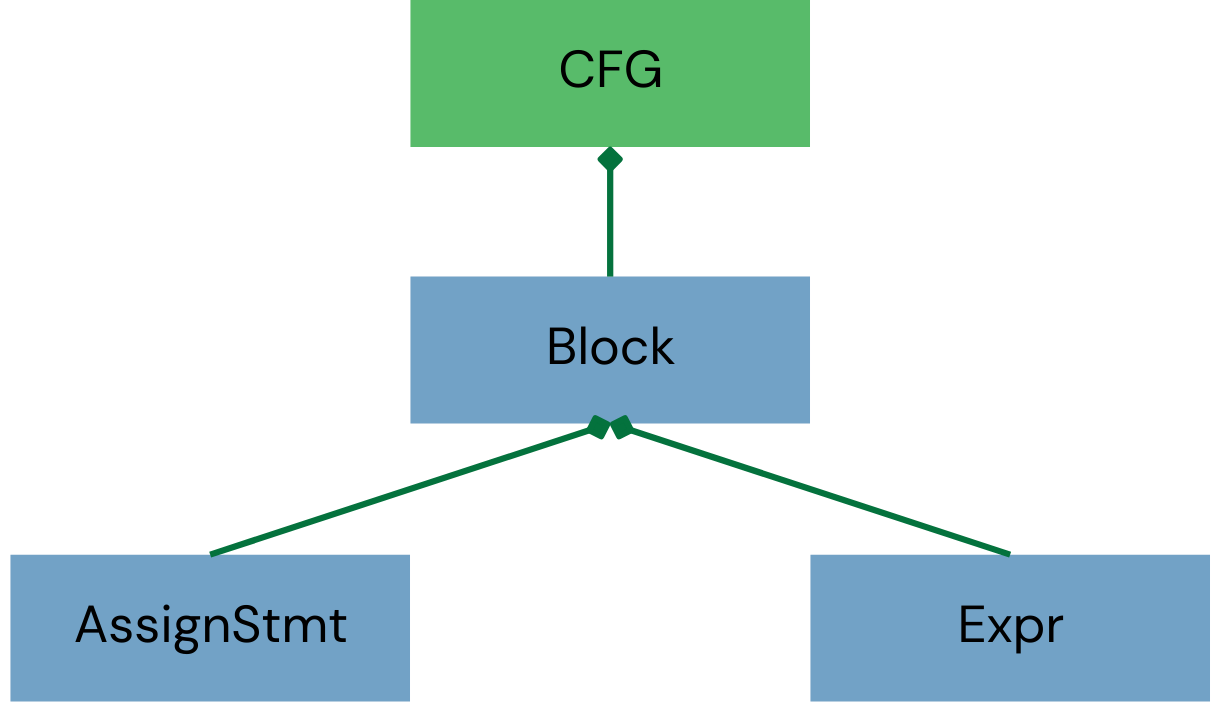
\includegraphics[width = 0.5 \textwidth]{img/cfg.png}
  \caption{The structure of a CFG}
  \label{figure:cfg-structure}
\end{figure}

\begin{figure}[ht]
  \centering
  \begin{minipage}[t]{0.4\textwidth} % Adjust the width here
    \begin{lstlisting}[language=Python]
data = '''
main : function void() {
a : array[5] of integer = {5,4,3,2,1};
tmp : integer;
for (i = 0; i < 4; i = i + 1){
  for (j = i+1; j < 5; j = j + 1) {
    if (a[i] > a[j]) {
      tmp = a[i];
      a[i] = a[j];
      a[j] = tmp;
    }
  }
}
}
'''
\end{lstlisting}
  \end{minipage}
  \hfill
  \begin{minipage}[t]{0.55\textwidth}
    \begin{lstlisting}[language=Python]
'''
Program([
  Func(main, void, [], None, 
    Block([
      Assign(a, [5, 4, 3, 2, 1]),
      Assign(i, 0.0),
      While(BinExpr(<, i, 4), 
        Block([
          Assign(j, BinExpr(+, i, 1)),
          While(BinExpr(<, j, 5), 
            Block([
              If(BinExpr(>, ArrayCell(a, [i]), ArrayCell(a, [j])), 
              Assign(tmp, ArrayCell(a, [i]))),
              Assign(ArrayCell(a, [i]), ArrayCell(a, [j])),
              Assign(ArrayCell(a, [j]), tmp),
              Assign(j, BinExpr(+, j, 1))
            ])),
          Assign(i, BinExpr(+, i, 1))]))]))
])
'''
\end{lstlisting}
  \end{minipage}
  \vfill
  \begin{minipage}[t]{\textwidth}
    \centering
    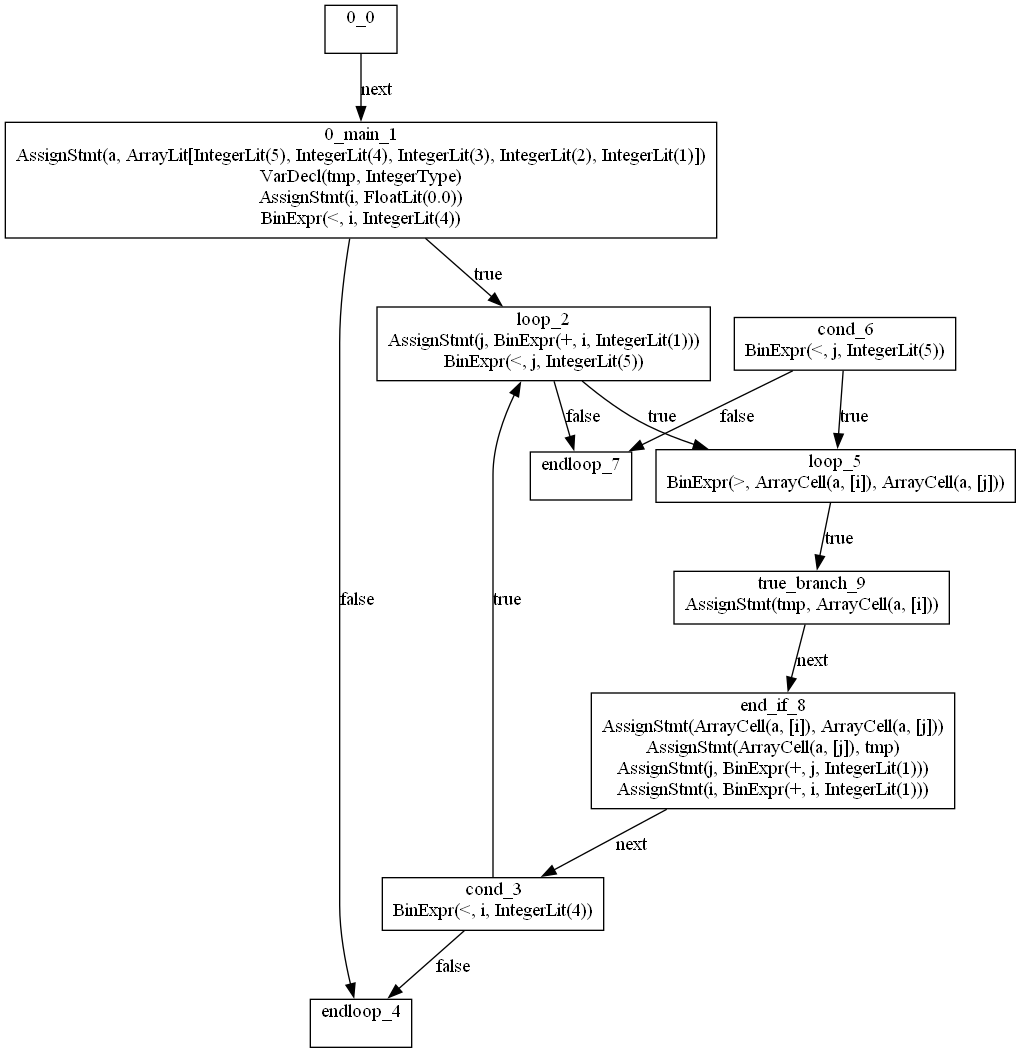
\includegraphics[width=0.8\textwidth]{img/cfg-example.png}
  \end{minipage}
  \caption{A MT22 program, its refactored AST and its corresponding CFG (rendered with Graphiz)}
\end{figure}
